\documentclass[10pt,a4paper,titlepage]{jreport} % ドキュメントクラスを1つに統一


\usepackage[top=25truemm,bottom=25truemm,left=20truemm,right=20truemm]{geometry} % 余白設定
\usepackage[dvipdfmx]{graphicx} % 画像の挿入
\usepackage{listings} % コードリスト用
\usepackage{jlisting} % 日本語対応のリスト用
\usepackage{float}
\usepackage{jverb} % 日本語のベタ打ち
\usepackage{booktabs}
\usepackage{pgfplots} % グラフ描画用パッケージ
\pgfplotsset{compat=1.18} % バージョン指定

\parindent = 0pt % 段落の字下げを無効化

\usepackage{titlesec}
\usepackage{etoolbox}
\makeatletter
\patchcmd{\chapter}{\if@openleft\cleardoublepage\else\if@openright\cleardoublepage\else\clearpage\fi\fi}{}{}{}
\makeatother
\lstset{breaklines=true, postbreak=\mbox{$\hookrightarrow$}\space, keepspaces=true, escapeinside={\%*}{*)}}

\titleformat{\chapter}[hang] % 章のフォーマットを変更
  {\normalfont\huge\bfseries} % フォント設定
  {\thechapter} % 番号部分の表示形式
  {1em} % 番号とタイトルの間のスペース
  {} % タイトルの前に入れる内容(ここでは空)

\usepackage{amsmath}
\usepackage{xcolor}

\lstset{
  language=Matlab,              % 言語はMATLAB
  basicstyle=\ttfamily,   % フォントは等幅、サイズ小さめ
  keywordstyle=\color{blue},    % キーワード(function, endとか)を青
  commentstyle=\color{green!50!black}, % コメントを深緑
  stringstyle=\color{red!70!black},    % 文字列('...')を赤系
  numbers=left,                 % 行番号を左に表示
  numberstyle=\tiny\color{gray},% 行番号をグレーで小さく
  stepnumber=1,                 % 毎行行番号つける
  numbersep=10pt,               % コードとの間隔
  backgroundcolor=\color{gray!10}, % 背景うっすらグレー
  frame=single,                 % 枠をつける
  rulecolor=\color{black},      % 枠線は黒
  breaklines=true,              % 長い行を折り返す
  breakatwhitespace=false,      % スペースでだけ折り返すか(falseにして自然な折り返し)
  showspaces=false,             % スペースは特別に表示しない
  showstringspaces=false,       % 文字列中のスペースも普通に表示
  tabsize=2                     % タブ幅2
}

\title{R101/R102 演習3-2} % タイトル
\author{
  学生番号:242C2016  氏名:奥村直 \\
  \\
  知的システム工学科システム制御コース
  } % 著者
\date{\today} % 日付
\begin{document}
\maketitle

\chapter{演習3-2}

\section{listing3.1の確認}

\begin{lstlisting}[caption=Listing3.1の確認]

% mobile_robot_params.m
% Configuration parameters for mobile robot simulation

% Robot physical parameters - fixed, not intended to be changed
params.wheel_radius = 0.05;  % radius of wheel [m]
params.wheel_distance = 0.23;  % distance between wheels [m]
params.body_length = 0.3;    % length of robot body [m]
params.body_width = 0.3;     % width of robot body [m]

% Simulation parameters
params.sim_time = 40;        % simulation time [s]
params.ode_max_step = 1e-1;  % maximum step size for ODE solver

% Animation parameters
params.draw_mode = 1;        % 0: update existing plot, 1: create new plot each frame
params.ani_sample = 100;     % animation sampling rate (higher = slower animation)
params.field_size = 3;       % size of the field for visualization [m]

% Motion parameters - different exercises
% Exercise 1: Constant wheel velocities
ex1.left_wheel_vel = 1.0;   % left wheel angular velocity [rad/s]
ex1.right_wheel_vel = 1.0;  % right wheel angular velocity [rad/s]

% Exercise 2: Circular motion
ex2.period = 40;            % period [s]
ex2.radius = 1.0;           % radius of rotation [m]

% Exercise 3: Figure-8 motion
ex3.period = 20;            % period for half of figure-8 [s]
ex3.radius = 1.0;           % radius of rotation [m]

% Exercise 4: Square path
ex4.period = 10;            % period for each segment [s]
ex4.side_length = 2.0;      % length of one side of square [m]

% Motion type selection (1, 2, 3, or 4)
% Change this value to select different motion types:
% 1: Constant Wheel Velocities
% 2: Circular Motion
% 3: Figure-8 Motion
% 4: Square Path
params.motion_type = 1;

% Combine all exercise parameters
params.ex1 = ex1;
params.ex2 = ex2; 
params.ex3 = ex3;
params.ex4 = ex4;

\end{lstlisting}

上記ソースコードより、
すでに用意されていたListing3.1のファイルを開いてparams.motion_typeが1で初期化されていることを確認した。

\section{プログラムの修正}

テキスト(第3章)中に指示された箇所を修正して状態方程式を追加した。シミュレーションの画像とグラフを出力した。

\begin{lstlisting}[caption=modified_dynamics_mobile_robot.m]

function [dxdt, wheel_vel] = dynamics_mobile_robot(t, x, params)
% Dynamics of mobile robot
% Inputs:
%   t - current time [s]
%   x - state vector [x_position; y_position; theta_orientation]
%   params - structure containing robot parameters
% Outputs:
%   dxdt - time derivative of state vector
%   wheel_vel - [left_wheel_velocity, right_wheel_velocity]

% Extract state
xc = x(1);      % x-position [m]
yc = x(2);      % y-position [m]
theta = x(3);   % orientation [rad]

% Extract robot parameters
r = params.wheel_radius;     % radius of wheel [m]
d = params.wheel_distance;   % distance between wheels [m]

% Get wheel velocities directly from the controller
[dphi_l, dphi_r] = mobile_robot_controller(t, x, params);
v = (r/2)*(dphi_l + dphi_r);
omega = (r/d)*(dphi_r - dphi_l);
% State equations
% TODO: Fix this
dx1dt = v * cos(theta);
dx2dt = v * sin(theta);
dx3dt = omega;

% Output
dxdt = [dx1dt; dx2dt; dx3dt];
wheel_vel = [dphi_l, dphi_r];
end

\end{lstlisting}

\begin{figure}[H] % Hで「ここに出せ」と指定(\usepackage{here}が必要)
  \centering
  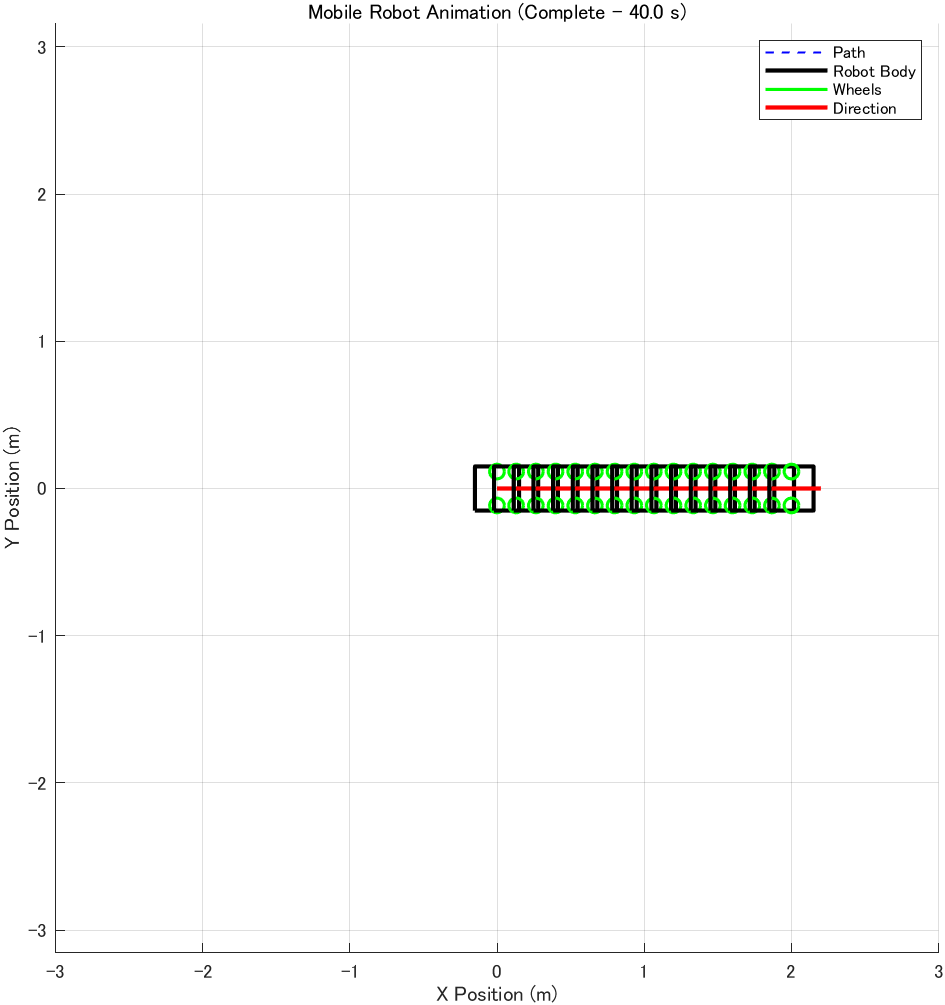
\includegraphics[width=0.6\linewidth]{242C2016_NaoOkumura_3_2_a.eps} % 拡張子付きOK(dvipdfmx前提)
\end{figure}

\begin{figure}[H] % Hで「ここに出せ」と指定(\usepackage{here}が必要)
  \centering
  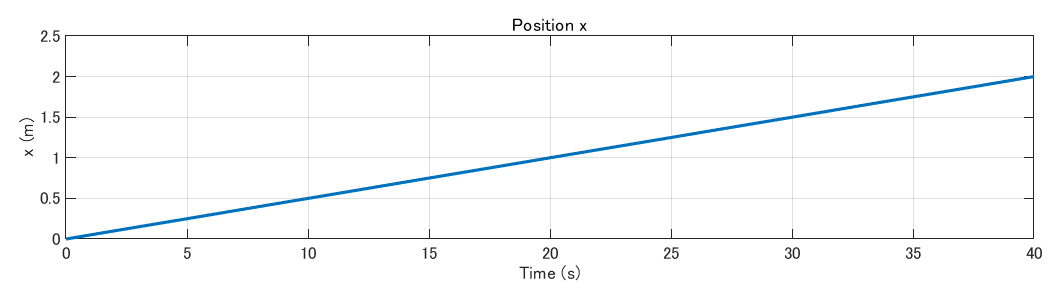
\includegraphics[width=0.6\linewidth]{242C2016_NaoOkumura_3_2_b.eps} % 拡張子付きOK(dvipdfmx前提)
\end{figure}

\begin{figure}[H] % Hで「ここに出せ」と指定(\usepackage{here}が必要)
  \centering
  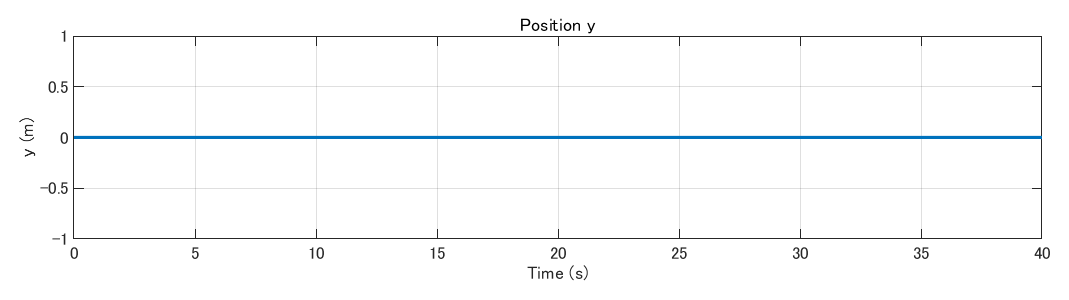
\includegraphics[width=0.6\linewidth]{242C2016_NaoOkumura_3_2_c.eps} % 拡張子付きOK(dvipdfmx前提)
\end{figure}

\begin{figure}[H] % Hで「ここに出せ」と指定(\usepackage{here}が必要)
  \centering
  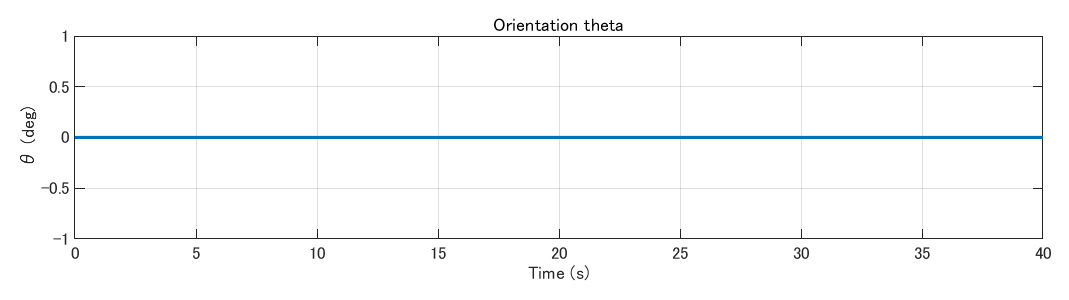
\includegraphics[width=0.6\linewidth]{242C2016_NaoOkumura_3_2_d.eps} % 拡張子付きOK(dvipdfmx前提)
\end{figure}

\chapter{参考文献}

- テキスト(第3章)

\end{document}